\documentclass[11pt,letterpaper]{article}
\usepackage[T1]{fontenc}
\usepackage{mathptmx}
\usepackage[scaled=0.90]{helvet}
\usepackage{microtype}
\usepackage[margin=1in]{geometry}
\usepackage{amsmath,amssymb,amsthm}
\usepackage{booktabs}
\usepackage{array}
\usepackage{tikz}
\usetikzlibrary{arrows.meta,positioning,calc}
\usepackage{enumitem}
\usepackage{titlesec}
\usepackage{fancyhdr}
\usepackage{framed}
\usepackage{xcolor}
\usepackage[colorlinks=true,linkcolor=black,urlcolor=black,citecolor=black]{hyperref}

\definecolor{shadecolor}{gray}{0.93}
\setcounter{tocdepth}{2}

\pagestyle{fancy}
\fancyhf{}
\lhead{\small ECON 601 \textbullet{} Lecture 3: Indirect Utility}
\rhead{\small\thepage}
\renewcommand{\headrulewidth}{0.4pt}

\theoremstyle{definition}
\newtheorem{defn}{Definition}
\theoremstyle{plain}
\newtheorem{thm}{Theorem}
\newtheorem{prop}{Proposition}
\newtheorem{lem}{Lemma}

\newcommand{\src}[1]{{\small\textsf{(#1)}}}
\newcommand{\fwd}[1]{\textsf{\textbf{$\rightarrow$ #1:}}}
\newcommand{\bwd}[1]{\textsf{\textbf{$\leftarrow$ #1:}}}
\newcommand{\wpref}{\succsim}
\newcommand{\spref}{\succ}
\newcommand{\Rn}{\mathbb{R}^n_+}
\newcommand{\MRS}{\mathrm{MRS}}
\newcommand{\skipnote}{\noindent{\small\textsf{Proof. Skippable on a first read.}}\par\smallskip}

\setlist{itemsep=1pt,topsep=3pt}

\title{\vspace{-2.2em}\textbf{Lecture 3: Indirect Utility}\\[0.3em]
\large ECON 601, with the ideas before the formulas}
\author{}
\date{}

\begin{document}
\maketitle
\vspace{-3em}
\begin{center}
\small \textbf{How to read this.} Each section opens with a concrete situation and a plain-English
claim. The formal statement follows. Proofs sit in ruled blocks and can be skipped entirely on a
first pass; nothing later depends on having read them. One consumer with real numbers runs through
the whole document.\\[0.4em]
Sources: Lectures 1--5 (L1--L5), Review Sessions 1--3 (RS1--RS3), Jehle \& Reny 3rd ed.\ (J\&R).
\end{center}
\vspace{0.8em}

{\small\tableofcontents}
\vspace{1em}

\section{Why any of this exists}

\subsection{The problem: comparing situations, not baskets}

Lecture 1 built a way to compare two shopping baskets. Lecture 2 found the best affordable basket.
Neither lets you answer the question that policy actually asks, which is whether a person is better
off in one \emph{situation} than another.

Suppose your city is choosing between two proposals. One gives every resident an extra \$20 a week.
The other caps the price of coffee at \$1.50. These are not baskets; they are environments, and they
change what is affordable in different ways. To compare them you need one number per environment
that says how well off a person ends up. That number is what Lecture 3 constructs, and it is called
indirect utility.

There is a second reason, and it is the deeper one. Prices, incomes and purchases are observable.
Preferences are not. Lecture 3 ends with a formula that reads the shopping list off the welfare
number, which means you can work backwards from how people are affected by price changes to what
they buy, without ever seeing inside anyone's head.

\begin{center}
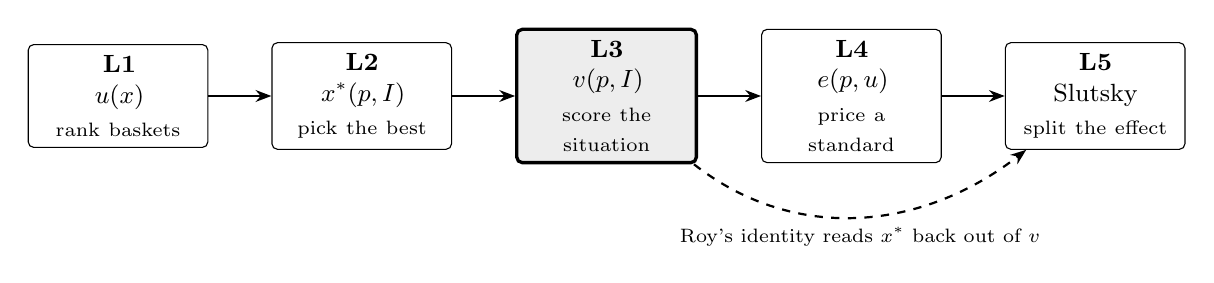
\begin{tikzpicture}[
  node distance=8mm,
  box/.style={draw,rounded corners=2pt,align=center,inner sep=4pt,font=\small,minimum height=12mm,text width=20mm},
  focus/.style={box,very thick,fill=shadecolor},
  arr/.style={-{Stealth[length=2mm]},thick}
]
\node[box] (l1) {\textbf{L1}\\$u(x)$\\[1pt]{\scriptsize rank baskets}};
\node[box,right=of l1] (l2) {\textbf{L2}\\$x^*(p,I)$\\[1pt]{\scriptsize pick the best}};
\node[focus,right=of l2] (l3) {\textbf{L3}\\$v(p,I)$\\[1pt]{\scriptsize score the situation}};
\node[box,right=of l3] (l4) {\textbf{L4}\\$e(p,u)$\\[1pt]{\scriptsize price a standard}};
\node[box,right=of l4] (l5) {\textbf{L5}\\Slutsky\\[1pt]{\scriptsize split the effect}};
\draw[arr] (l1) -- (l2);
\draw[arr] (l2) -- (l3);
\draw[arr] (l3) -- (l4);
\draw[arr] (l4) -- (l5);
\draw[arr,dashed] (l3) to[out=-38,in=-142] node[below,font=\scriptsize]{Roy's identity reads $x^*$ back out of $v$} (l5);
\end{tikzpicture}
\end{center}

\subsection{Our consumer, for the rest of the document}

Every claim below is illustrated on one person. She has \$120 a week to spend on coffee and lunch.
Coffee is \$2, lunch is \$3. Her tastes are Cobb-Douglas with equal weight on the two,
$u = \sqrt{x_1 x_2}$, which means she splits her money evenly between them \src{RS3 Q3.4}.

\begin{center}
\begin{tabular}{@{}lll@{}}
\toprule
\textbf{Symbol} & \textbf{Her numbers} & \textbf{What it is} \\
\midrule
$I$ & \$120 & weekly budget \\
$p_1, p_2$ & \$2, \$3 & price of a coffee, price of a lunch \\
$x_1^*, x_2^*$ & 30, 20 & what she buys: 30 coffees, 20 lunches \\
$v$ & 24.49 & her standard of living at these prices and this income \\
$\lambda^*$ & 0.204 & what one more dollar is worth to her, in utility \\
\bottomrule
\end{tabular}
\end{center}

Two warnings about that table. The 24.49 is not dollars and not anything else physical; it is a score
on an arbitrary scale, and \S\ref{sec:q6} explains what can and cannot be done with it. The 0.204 is
equally arbitrary. The 30 and the 20 are real.

\subsection{The six questions, and what each one costs}

Lecture 3 asks six questions in order, and it is worth knowing in advance which assumption each one
is spending.

\begin{center}
\begin{tabular}{@{}p{0.42\textwidth} p{0.30\textwidth} p{0.20\textwidth}@{}}
\toprule
\textbf{Question} & \textbf{What it costs} & \textbf{Where} \\
\midrule
Q1. Is there a number at all? & continuity of $u$, inherited from L2 & \S\ref{sec:q1} \\
Q2. What can we say about it knowing nothing about the person? & nothing about $u$ & \S\ref{sec:q2} \\
Q3. Are two extreme situations better than the average of them? & still nothing about $u$ & \S\ref{sec:q3} \\
Q4. Does the number move smoothly? Does behaviour? & continuity for the number; strict curvature for behaviour & \S\ref{sec:q4} \\
Q5. How do we differentiate it without solving the problem again? & differentiability & \S\ref{sec:q5} \\
Q6. Can we read the shopping list back out of it? & all three of the above & \S\ref{sec:q6} \\
\bottomrule
\end{tabular}
\end{center}

\textbf{The flat middle is the point.} Q2 and Q3 cost nothing about preferences. They hold for a
person with any tastes whatsoever, because they follow from how the set of affordable baskets moves
when prices and income move. If you find yourself reaching for a property of $u$ while proving one
of these, you have gone wrong. The lecture says so explicitly about Q3 \src{L3 p.3}.

\subsection{Every symbol in plain words}

Keep this next to you while reading the lecture notes.

\begin{center}
\begin{tabular}{@{}ll@{}}
\toprule
\textbf{Symbol} & \textbf{Say it like this} \\
\midrule
$u(x)$ & how good this particular basket is, on an arbitrary scale \\
$B(p,I)$ & everything she can afford \\
$x^*(p,I)$ & her shopping list \\
$v(p,I)$ & her standard of living, given these prices and this income \\
$\lambda^*$ & the exchange rate between utility and dollars \\
$\mathcal{L}$ & the problem rewritten so that overspending is priced instead of banned \\
$e(p,u^0)$ & what a fixed standard of living costs at these prices \src{L4} \\
$x^h(p,u^0)$ & what she would buy if compensated to keep her standard fixed \src{L4} \\
\bottomrule
\end{tabular}
\end{center}

\textbf{Why the word ``indirect''.} A direct utility function takes a basket and returns a score.
The indirect one takes prices and income, works out the basket for you, and returns the score of
that. It is the same scale, reached by a longer route.

\section{What Lectures 1 and 2 hand over}

\subsection{The delivery manifest}

Lecture 3 is not a fresh start. Almost everything it uses arrived earlier.

\begin{center}
\begin{tabular}{@{}p{0.30\textwidth} p{0.36\textwidth} p{0.26\textwidth}@{}}
\toprule
\textbf{Earlier result} & \textbf{What it becomes here} & \textbf{Used by} \\
\midrule
$B$ is non-empty, convex, compact \src{L2 p.2} & the only thing Q2 and Q3 are about & Q1, Q2, Q3 \\
Weierstrass with continuous $u$ \src{L2 p.2} & a best basket exists, so the score exists & Q1 \\
Demand is HD0 in $(p,I)$ \src{L2 p.4} & the score is HD0 too & Q2 \\
Strict curvature gives one best basket \src{L2 p.3} & behaviour moves smoothly, and Roy has a number to return & Q4, Q6 \\
Strictly increasing $u$ makes the budget bind, $\lambda^* > 0$ \src{L2 p.7} & the denominator in Roy's identity is not zero & Q5, Q6 \\
The Lagrangian \src{L2 p.7} & the thing we differentiate in Q5 & Q5, Q6 \\
Euler's theorem \src{L2 p.3}, \src{RS3 Q1.2} & a free restriction on the derivatives of the score & Q2, and the check in \S\ref{sec:q6} \\
$u$ is ordinal \src{L1 p.5} & the score is \emph{not} ordinal, but the list read out of it is & Q1, Q6 \\
\bottomrule
\end{tabular}
\end{center}

\subsection{Three facts that shape every answer}

\textbf{Prices and income touch only the constraint, never the objective.} Write the problem out and
look at where $p$ and $I$ appear. The thing being maximized, $u(x)$, has no price in it anywhere. All
the dependence on the environment runs through the single set of affordable baskets. That one
observation proves three separate results in \S\ref{sec:q2} and \S\ref{sec:q3}, and Lecture 4 reuses
it twice more \src{L4 p.2}.

\textbf{$\lambda^*$ is strictly positive when more is always better.} Lecture 2 got this from the
first-order conditions \src{L2 p.7}: if an extra unit of some good always helps, then an extra dollar
is worth something strictly positive. For our consumer that number is 0.204. In Lecture 3 the same
number turns out to be the derivative of her standard of living with respect to income, and
\S\ref{sec:q6} divides by it.

\textbf{Only strict curvature gives one best basket.} Weak curvature permits a whole line of equally
good baskets, which is what happens with two goods the consumer regards as interchangeable
\src{L2 pp.3--4}. That case returns in \S\ref{sec:q4} as the example where the standard of living is
smooth and behaviour is not.

\begin{snugshade}
\noindent\textbf{Background you can leave alone.} The complementary-slackness bookkeeping of the
Kuhn-Tucker conditions \src{L2 pp.6--7}, since Lecture 3 uses only the single fact
$\lambda^* > 0$. The corner-solution example at \src{L2 pp.8--10}. The axioms of Lecture 1, which
enter only as the standing assumption that a continuous $u$ exists. Do not leave alone Lecture 1's
point that $u$ is ordinal, because \S\ref{sec:q6} turns on it.
\end{snugshade}
\section{A number for how well off you are}
\label{sec:q1}

\subsection{The scene: two policies, one comparison}

Back to the city council. Proposal A gives our consumer an extra \$20 a week. Proposal B caps coffee
at \$1.50. Work out what she does under each.

\begin{center}
\begin{tabular}{@{}llll@{}}
\toprule
 & \textbf{Her budget and prices} & \textbf{She buys} & \textbf{Her score} \\
\midrule
Now & \$120; coffee \$2, lunch \$3 & 30 coffees, 20 lunches & 24.49 \\
Proposal A & \$140; coffee \$2, lunch \$3 & 35 coffees, 23.3 lunches & 28.58 \\
Proposal B & \$120; coffee \$1.50, lunch \$3 & 40 coffees, 20 lunches & 28.28 \\
\bottomrule
\end{tabular}
\end{center}

A wins, but barely, and you could not have called it by eye. Under B she gets more coffee; under A
she gets more of both but less coffee than B gives her. The baskets are not comparable by inspection,
and the whole reason for the score is that it makes them comparable.

\subsection{What has to be true for the number to exist}

\textbf{The claim in plain words.} If she can always say which of two baskets she prefers, if her
preferences do not jump, and if every good costs something, then there is a best affordable basket
and it has a score.

\begin{defn}[Indirect utility]
\[
v(p,I) = \max_{x \ge 0} \ u(x) \quad \text{subject to} \quad p \cdot x \le I,
\qquad v(p,I) = u\big( x^*(p,I) \big). \qquad \src{L3 p.1}, \src{RS3 Def.\ 2.1}
\]
\end{defn}

Writing $\max$ is a claim and not a notation. Two things could go wrong. She might improve forever
without arriving, and she might approach a best score without reaching it.

\begin{prop}[Existence] If $u$ is continuous, $p \gg 0$ and $I > 0$, then $v(p,I)$ exists.
\src{L2 p.2}, \src{L3 p.1}
\end{prop}

\skipnote
\begin{leftbar}
\small
Lecture 2 shows $B = \{ x \ge 0 \mid p \cdot x \le I \}$ is non-empty, convex and compact
\src{L2 p.2}. A continuous function on a compact set attains its maximum, so a best basket exists
and $u$ of it is a number.
\end{leftbar}

\bwd{L2} Compactness came from $p \gg 0$: if every good has a strictly positive price, then spending
at most \$120 caps how much of anything she can hold. That is the only job $p \gg 0$ does here, and
\S\ref{sec:q1}.4 shows what happens without it.

\subsection{The tie problem, and why it is not a problem}

Here is a worry that the lecture passes over and that is worth a minute. Suppose two different
baskets are both best. Then $x^*$ is not a single basket, and the formula $v = u(x^*)$ looks
ambiguous: which one do you plug in?

\textbf{The answer is that it does not matter.} If two baskets are both best, they are tied, and tied
means the same score by definition. Formally, if $\hat x$ and $\hat{\hat x}$ both maximize, then
$u(\hat x) \ge u(\hat{\hat x})$ and $u(\hat{\hat x}) \ge u(\hat x)$, so the two are equal.

This is why the rest of the lecture can proceed without assuming the best basket is unique. The score
is always a well-defined single number even when behaviour is not pinned down, and \S\ref{sec:q4} is
built on exactly that gap.

\subsection{What breaks: free coffee}

Suppose the council instead makes coffee free. Now she can have as much as she likes, and since more
coffee always helps her a little, there is no best basket. She would take a hundred coffees, then a
thousand, and never arrive.

That is the failure of $p \gg 0$, and the chain is worth tracing. Free coffee means her affordable
set is unbounded, which means it is not compact, which means Weierstrass does not apply, which means
there is no maximum, which means $v$ is not defined \src{L2 p.2}. Every later result in this lecture
quietly assumes this did not happen.

\subsection{The one place the score behaves worse than the shopping list}

Lecture 1 made a great deal of the fact that utility numbers are arbitrary labels: if $u$ works, so
does $1000u$, or $\ln u$, or any strictly increasing relabeling \src{L1 p.5}. Her shopping list
survives that relabeling, because relabeling does not change which basket is best.

The score does not survive it. Our consumer's 24.49 becomes 24{,}490 if we use $1000u$, or 3.20 if
we use $\ln u$. Same person, same coffee, same lunches, different number \src{RS3 p.4, Remark 2}.

So $v$ is a comparison device and not a measurement. Saying she scores 28.58 under Proposal A and
28.28 under Proposal B is meaningful, because the ranking survives relabeling. Saying A is 1 percent
better is not, because that ratio does not. This turns out to be exactly the right amount of
information, and \S\ref{sec:q6} shows why.

\fwd{L4} The mirror problem asks what a fixed standard of living costs, and its answer $e(p,u^0)$ is
measured in dollars, which is not an arbitrary scale \src{L4 p.1}. That single difference explains
most of the differences between the two lectures' formulas, and \S\ref{sec:q6} spells it out.

\section{Dropping three zeros from the currency}
\label{sec:q2}

\subsection{The scene}

In 2005 Turkey removed six zeros from the lira. A loaf of bread that cost 1{,}500{,}000 lira on
Monday cost 1.50 on Tuesday, and every wage was rescaled the same way. Nobody's breakfast changed.

Run it on our consumer. Before: \$120, coffee \$2, lunch \$3, buying 30 and 20. Multiply everything
by a thousand: \$120{,}000, coffee \$2{,}000, lunch \$3{,}000. She still buys 30 coffees and 20
lunches, and she is neither better nor worse off. Her score is unchanged at 24.49.

\subsection{The score does not notice}

\textbf{The claim in plain words.} Her standard of living depends on what she can afford, and
multiplying all prices and her income by the same number leaves the set of affordable baskets exactly
as it was. Not a similar set. The identical set.

Everything in this section and the next rests on two small facts about that set.

\begin{lem}[A smaller menu cannot have a better best item] \label{lem:mv}
If $B' \subseteq B$ then $\max_{x \in B'} u(x) \le \max_{x \in B} u(x)$.
\end{lem}

\skipnote
\begin{leftbar}
\small
Let $x'$ be best in $B'$. Since $B' \subseteq B$, that basket is available in $B$ too, so the best in
$B$ scores at least as well.
\end{leftbar}

\begin{lem}[How the affordable set moves] \label{lem:bmove}
For $p \gg 0$, $I > 0$, $t > 0$: \ (a) $B(tp, tI) = B(p,I)$; \ (b) if $p^0 \ge p^1$ then
$B(p^0, I) \subseteq B(p^1, I)$; \ (c) if $I^0 \le I^1$ then $B(p, I^0) \subseteq B(p, I^1)$.
\end{lem}

\skipnote
\begin{leftbar}
\small
(a) Since $t > 0$, the inequality $tp \cdot x \le tI$ can be divided by $t$ and becomes
$p \cdot x \le I$. Same inequality, same set \src{L3 p.1}.

(b) If $x \ge 0$ and $p^0 \cdot x \le I$, then because every price fell or stayed put,
$p^1 \cdot x \le p^0 \cdot x \le I$. The step needs $x \ge 0$: you cannot hold a negative quantity of
a good whose price dropped.

(c) Immediate, since $p \cdot x \le I^0 \le I^1$.
\end{leftbar}

\begin{prop}[Property 1] \label{prop:hd0}
$v(tp, tI) = v(p,I)$ for all $t > 0$. \src{L3 p.1}
\end{prop}

\skipnote
\begin{leftbar}
\small
The lecture states this with no proof at all. By Lemma \ref{lem:bmove}(a) the two problems have the
same feasible set, and the objective $u(x)$ contains no prices and no income. Two maximizations with
the same objective over the same set are the same maximization, so their values agree.
\end{leftbar}

\textbf{This is an assumption, not a tautology.} The model was built so that the consumer has no
money illusion, and real people demonstrably do. They accept a real pay cut delivered by inflation
and refuse the identical cut delivered in nominal terms; they anchor on the price a coffee used to
be. Knowing exactly which line produces the property, the line where $t$ divides out of the budget
constraint, is what lets you say something sensible when the model and the behaviour disagree.

\subsection{More money helps; cheaper coffee sometimes does nothing}

\textbf{The claim in plain words.} Raising a price can never make her better off and giving her more
money can never make her worse off. But only one of these is guaranteed to have a strict effect.

\begin{prop}[Property 2] \label{prop:mono}
$v$ is decreasing in each price and increasing in income. If $u$ is strictly increasing, then $v$ is
\emph{strictly} increasing in income. \src{L3 p.1}, \src{J\&R Thm 1.6}
\end{prop}

\skipnote
\begin{leftbar}
\small
For prices: if $p^0 \ge p^1$, Lemma \ref{lem:bmove}(b) gives
$B(p^0,I) \subseteq B(p^1,I)$, and Lemma \ref{lem:mv} then gives $v(p^0,I) \le v(p^1,I)$. Income is
the same argument with part (c).

For the strict claim, let $I^1 > I^0$ and let $x^0$ be best at $I^0$. Then $p \cdot x^0 \le I^0 <
I^1$, so there is slack. Pick $\varepsilon > 0$ small enough that
$p \cdot (x^0 + \varepsilon \mathbf{1}) \le I^1$, which is possible because the left side is
continuous in $\varepsilon$ and starts strictly below $I^1$. That basket is affordable at $I^1$ and,
since more of everything is strictly better, scores above $x^0$. So $v(p,I^1) > v(p,I^0)$.
\end{leftbar}

\textbf{Where the asymmetry comes from, concretely.} Consider a second consumer who drinks only
Pepsi, because Coke at \$1.02 costs more than Pepsi at \$1.01. Cut the price of Coke to \$1.00 and
she is better off. But cut it the other way, or raise Coke to \$1.50, and nothing at all happens to
her: she was not buying Coke and still is not. Her score does not move.

More income is different. There is no way to hand her money and have it do nothing, as long as some
good is worth buying more of. That is why the price claim is stated weakly and the income claim
strictly, and the difference matters in \S\ref{sec:q6}, where we divide by the income derivative.

\subsection{What breaks: a person who already has everything she wants}

Take a consumer with an ideal weekly basket, say exactly 4 coffees and 3 lunches, and who is made
worse off by deviating in either direction \src{RS2 Q2.3}. At \$120 a week she buys her ideal basket
for \$17, leaves \$103 on the table, and hands her another \$20 and her score does not move at all.

So the strict half of Proposition \ref{prop:mono} genuinely needs the hypothesis that more is always
better. For this consumer $\partial v / \partial I = 0$, and \S\ref{sec:q6} shows that this is
precisely the case where the main result of the lecture fails.

\subsection{A free restriction, and what it says}

Because the score does not notice a currency redenomination, its derivatives are not free to be
anything. Euler's theorem \src{L2 p.3}, \src{RS3 Q1.2} turns that global statement into one equation
at each point:
\begin{equation} \label{eq:eulerv}
\sum_{i} \frac{\partial v}{\partial p_i} \, p_i \ + \ \frac{\partial v}{\partial I} \, I \ = \ 0 .
\end{equation}

On our consumer the three terms are
\[
\underbrace{(-6.12)(2)}_{\text{coffee}} \ + \ \underbrace{(-4.08)(3)}_{\text{lunch}} \ + \
\underbrace{(0.204)(120)}_{\text{income}}
\ = \ -12.25 - 12.25 + 24.49 \ = \ 0 .
\]

\textbf{What that means.} Doubling every price would hurt her by 24.49 units of score, split between
the two goods. Doubling her income would help her by exactly 24.49. Doing both at once is a
redenomination and changes nothing, so the two effects must cancel exactly. The equation is that
cancellation, written down.

\fwd{L5} The same restriction written in percentage terms becomes the elasticity identities of
Lecture 5, $\sum_j s_j \varepsilon_{j,i} = -s_i$ and $\sum_j s_j \eta_j = 1$ \src{L5 p.9}. Those are
testable on real purchase data, and if an estimated demand system violates them, the data are outside
consumer theory.
\section{Two countries and the one in between}
\label{sec:q3}

\subsection{The scene: where would you rather live?}

Our consumer has \$120 a week wherever she goes. Three countries, differing only in prices.

\begin{center}
\begin{tabular}{@{}lllc@{}}
\toprule
 & \textbf{Prices} & \textbf{She buys} & \textbf{Her score} \\
\midrule
Country A & coffee \$2, lunch \$6 & 30 coffees, 10 lunches & 17.32 \\
Country B & coffee \$6, lunch \$2 & 10 coffees, 30 lunches & 17.32 \\
Country C, halfway between & coffee \$4, lunch \$4 & 15 coffees, 15 lunches & \textbf{15.00} \\
\bottomrule
\end{tabular}
\end{center}

The country in the middle is worse than both of the extremes. Not between them. Worse than both.

\textbf{Why, in one sentence.} In A she leans into coffee and in B she leans into lunch, and in each
case the thing she leans into is cheap. C takes away the option to lean.

The everyday version: a city where rent is high and food is cheap lets you live small and eat out
constantly. A city where rent is cheap and food is expensive lets you live large and cook. The city
where both are middling denies you both strategies, and you can end up worse off than in either
extreme even though nothing there is especially expensive.

\subsection{The claim in plain words}

Averaging two price situations never produces something better than the better of the two. It can
produce something worse than both. That is the property called quasi-convexity, and it is the only
genuinely surprising result in the lecture. The lecture itself calls it perhaps the least obvious
\src{L3 p.3}.

\textbf{What it is not about.} Nothing above used any fact about her tastes. She could like anything
at all and the result would still hold. The lecture says so directly, noting it is true whether or
not $u$ is quasi-concave \src{L3 p.3}. Everyone's instinct at this point is to reach for an axiom
on preferences, because Lecture 1 spent a whole section connecting curvature to preferences. There is
no preference hypothesis here.

\subsection{Why it happens: her three budget lines all cross at one point}

Draw the three countries in the space of baskets. Each is a budget line, and all three pass through
the same point.

\begin{center}
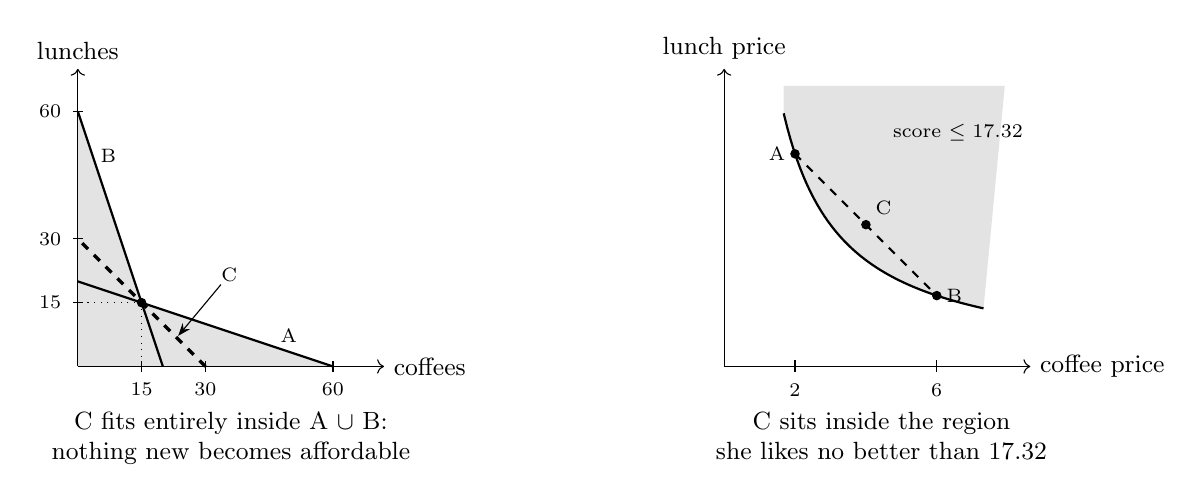
\begin{tikzpicture}[scale=1.08]
\begin{scope}
  \fill[black!11] (0,0) -- (3.0,0) -- (0,1.0) -- cycle;
  \fill[black!11] (0,0) -- (1.0,0) -- (0,3.0) -- cycle;
  \draw[->] (0,0) -- (3.6,0) node[right,font=\small] {coffees};
  \draw[->] (0,0) -- (0,3.5) node[above,font=\small] {lunches};
  \draw[thick] (3.0,0) -- (0,1.0);
  \draw[thick] (1.0,0) -- (0,3.0);
  \draw[very thick,dashed] (1.5,0) -- (0,1.5);
  \draw[dotted] (0.75,0.75) -- (0.75,0);
  \draw[dotted] (0.75,0.75) -- (0,0.75);
  \fill (0.75,0.75) circle (1.6pt);
  \foreach \p/\l in {0.75/15, 1.5/30, 3.0/60} {
    \draw (\p,-0.06) -- (\p,0.06); \node[font=\scriptsize,anchor=north] at (\p,-0.08) {\l};
    \draw (-0.06,\p) -- (0.06,\p); \node[font=\scriptsize,anchor=east] at (-0.08,\p) {\l};
  }
  \node[font=\scriptsize,fill=white,inner sep=1pt] at (2.48,0.36) {A};
  \node[font=\scriptsize,fill=white,inner sep=1pt] at (0.36,2.48) {B};
  \node[font=\scriptsize,fill=white,inner sep=1pt] (bt) at (1.78,1.08) {C};
  \draw[-{Stealth[length=1.6mm]}] (bt) -- (1.18,0.36);
  \node[font=\small,anchor=north,align=center] at (1.8,-0.42)
    {C fits entirely inside A $\cup$ B:\\ nothing new becomes affordable};
\end{scope}
\begin{scope}[xshift=7.6cm]
  \fill[black!11] plot[domain=0.70:3.05,samples=60] (\x,{2.0833/\x})
     -- (3.30,3.30) -- (0.70,3.30) -- cycle;
  \draw[->] (0,0) -- (3.6,0) node[right,font=\small] {coffee price};
  \draw[->] (0,0) -- (0,3.5) node[above,font=\small] {lunch price};
  \draw[thick,domain=0.70:3.05,samples=60] plot (\x,{2.0833/\x});
  \draw[dashed,thick] (0.833,2.5) -- (2.5,0.833);
  \fill (0.833,2.5) circle (1.6pt) node[left,font=\scriptsize] {A};
  \fill (2.5,0.833) circle (1.6pt) node[right,font=\scriptsize] {B};
  \fill (1.667,1.667) circle (1.6pt) node[above right,font=\scriptsize] {C};
  \draw (0.833,-0.07) -- (0.833,0.07); \node[font=\scriptsize,anchor=north] at (0.833,-0.09) {2};
  \draw (2.5,-0.07) -- (2.5,0.07); \node[font=\scriptsize,anchor=north] at (2.5,-0.09) {6};
  \node[font=\scriptsize] at (2.75,2.75) {score $\le 17.32$};
  \node[font=\small,anchor=north,align=center] at (1.85,-0.42)
    {C sits inside the region\\ she likes no better than 17.32};
\end{scope}
\end{tikzpicture}
\end{center}

Look at the left panel. Country C's budget line is strictly inside the union of A's and B's. Every
basket she could afford in C, she could already have afforded in A or in B. So nothing in C is new,
and the best thing available in C was already available in one of the extremes. That is the entire
argument, and everything below is that sentence made precise.

\begin{defn}[Quasi-convex] $f$ is quasi-convex if
$f(t z^1 + (1-t) z^2) \le \max\{ f(z^1), f(z^2) \}$ for all $z^1, z^2$ and $t \in [0,1]$,
equivalently if every set $\{ z : f(z) \le K \}$ is convex. \src{L3 p.3}
\end{defn}

\begin{thm}[Property 3] \label{thm:qcx}
$v(p,I)$ is quasi-convex in $(p,I)$. \src{L3 pp.3--4}, \src{J\&R Thm 1.6}
\end{thm}

The lecture proves the containment step and then asserts that it suffices. Both halves are below.

\skipnote
\begin{leftbar}
\small
\textbf{Step 1, the containment.} Write $p^t = t p^1 + (1-t)p^2$ and $I^t = t I^1 + (1-t) I^2$. Claim:
$B(p^t, I^t) \subseteq B(p^1,I^1) \cup B(p^2,I^2)$.

At $t = 0$ and $t=1$ this is trivial, so take $t \in (0,1)$ and suppose it fails. Then some basket
$x$ is affordable at the average prices but at neither extreme:
\[
p^1 \cdot x > I^1 \qquad \text{and} \qquad p^2 \cdot x > I^2 .
\]
Multiply the first by $t > 0$ and the second by $1-t > 0$, which preserves both, and add:
\[
\big( t p^1 + (1-t) p^2 \big) \cdot x > t I^1 + (1-t) I^2, \qquad \text{that is} \qquad
p^t \cdot x > I^t .
\]
So $x$ was not affordable at the average prices after all, a contradiction.

\textbf{Step 2, why that suffices.} The lecture stops at Step 1. Here is the rest. Let $x^t$ be her
best basket at the average prices, so $v(p^t,I^t) = u(x^t)$. By Step 1, $x^t$ was affordable either
at $(p^1,I^1)$ or at $(p^2,I^2)$. In the first case the best available at $(p^1,I^1)$ scores at least
$u(x^t)$, so $v(p^1,I^1) \ge v(p^t,I^t)$; in the second case the same for $(p^2,I^2)$. One of the two
holds, so
\[
v(p^t, I^t) \le \max\{ v(p^1,I^1), v(p^2,I^2) \},
\]
which is quasi-convexity.
\end{leftbar}

Notice there is nothing in that proof except arithmetic on the budget constraint. Her tastes never
appear. Existence of a best basket was used once, in Step 2, to have an $x^t$ to talk about.

\subsection{Two curvature words that look like a pair and are not}

Students routinely read ``quasi-concave $u$'' and ``quasi-convex $v$'' as two sides of one result.
They are unrelated, and the table is worth memorizing because exams test exactly this confusion.

\begin{center}
\begin{tabular}{@{}l l l@{}}
\toprule
 & \textbf{quasi-concave $u$} & \textbf{quasi-convex $v$} \\
\midrule
What is being averaged & two baskets & two price-income situations \\
Which set is convex & baskets at least as good & situations no better than $K$ \\
Where it comes from & an axiom on her preferences \src{L1 p.10} & arithmetic on the budget line \src{L3 p.4} \\
Does it need the other? & no & no \src{L3 p.3} \\
\bottomrule
\end{tabular}
\end{center}

\subsection{What breaks: a bulk discount}

The only substantive step in the proof was multiplying two inequalities by $t$ and $1-t$ and adding
them, and that needs the cost of a basket to be linear in prices.

Suppose instead coffee is \$2 each but \$1.50 each if you buy more than twenty. Now the cost of a
basket is not a straight line in the price, the addition step fails, and Country C need not fit
inside A $\cup$ B. Averaging two price schedules can genuinely open up something new. Quasi-convexity
is a fact about linear pricing, not a fact about consumers.

\fwd{L4} The cost of a fixed standard of living, $e(p,u^0)$, is \emph{concave} in prices, which is a
different word and a different mechanism \src{L4 p.3}. The practical difference is that concavity
signs second derivatives and quasi-convexity signs nothing, which is why the whole substitution-matrix
apparatus of Lecture 4 lives on that side and has no counterpart here. Do not read the two results as
a matched pair.

\section{Coke, Pepsi, and a one-cent price change}
\label{sec:q4}

\subsection{The scene}

A different consumer spends \$12 a week on soda and regards Coke and Pepsi as interchangeable, one
for one. She buys whichever is cheaper.

\begin{center}
\begin{tabular}{@{}lllc@{}}
\toprule
 & \textbf{Prices} & \textbf{She buys} & \textbf{Her score} \\
\midrule
Monday & Coke \$1.00, Pepsi \$1.01 & 12 Cokes, 0 Pepsis & 12.00 \\
Tuesday & Coke \$1.02, Pepsi \$1.01 & 0 Cokes, 11.88 Pepsis & 11.88 \\
\bottomrule
\end{tabular}
\end{center}

A two-cent price change moved her welfare by about one percent and flipped her entire cart. Her
behaviour is not a little different on Tuesday; it has no overlap at all with Monday.

\subsection{Welfare is smooth, behaviour need not be}

\textbf{The claim in plain words.} How well off she is depends only on the price of the cheaper
option, and that moves smoothly. \emph{Which} option is cheaper can flip on a penny.

This is not a curiosity. It is the reason the whole lecture is worth doing. Value functions are
better behaved than the choices that generate them, so if you want something that responds smoothly
to policy, track welfare and not behaviour.

\subsection{Berge's theorem, in plain words}

\begin{thm}[Berge] If the menu varies continuously with the parameters and the scoring is continuous,
then the best available score varies continuously. The identity of the winner need not.
\src{L3 p.4}, \src{J\&R Thm A2.21}
\end{thm}

The lecture's proof of continuity is the single word ``Berge'' \src{L3 p.4}, so the work is in
checking the hypotheses. Her affordable set is never empty, because doing nothing is always an
option; it is bounded, because every good costs something; and it slides continuously as prices and
income slide, again because prices are strictly positive so the intercepts $I/p_i$ stay finite. The
last of these is what fails if some price hits zero, and it is the same place compactness failed in
Lecture 2.

\begin{prop}[Property 4] If $u$ is continuous then $v(p,I)$ is continuous on $p \gg 0$, $I \ge 0$.
\src{L3 p.3}
\end{prop}

What Berge does \emph{not} give is continuity of what she buys. The Coke and Pepsi table shows the
gap is real and not an artifact of a weak proof.

\subsection{When behaviour is smooth too}

\textbf{The claim in plain words.} If there is only ever one best basket, then nudging prices can
only nudge the basket. The basket cannot be in two places at once, so it has nowhere to jump to.

Our first consumer is in this case. Cobb-Douglas tastes give exactly one best basket at every price,
and her demands $30 = 60/p_1$ and $20 = 60/p_2$ are smooth curves. The soda drinker is not: at a tie
she has a whole line of best baskets, and that is precisely where the jump happens.

\begin{prop}[The lecture's Proposition 3.1] \label{prop:xcont}
If $u$ is also strictly quasi-concave, so that the best basket is unique, then $x^*(p,I)$ is
continuous. \src{L3 p.4, ``Proof. Omitted.''}
\end{prop}

\skipnote
\begin{leftbar}
\small
Fix $(p^0,I^0)$ with $p^0 \gg 0$, $I^0 > 0$, and let $(p^n,I^n) \to (p^0,I^0)$. Write
$x^n = x^*(p^n,I^n)$.

\emph{The baskets stay in a bounded region.} Since $p^0 \gg 0$ there are $\delta > 0$ and $N$ with
$p^n_i \ge \delta$ for all $i$ and all $n \ge N$, and with $I^n \le I^0 + 1$. Then
$\delta x^n_i \le p^n \cdot x^n \le I^0 + 1$, so from $N$ onward every $x^n$ lies in the compact box
$[0, (I^0+1)/\delta]^n$.

\emph{Every convergent subsequence lands on the same basket.} Suppose $x^{n_k} \to \bar x$.
Affordability survives the limit: $p^{n_k} \cdot x^{n_k} \le I^{n_k}$ gives
$p^0 \cdot \bar x \le I^0$. Optimality survives too, using continuity of $u$ and then Property 4:
\[
u(\bar x) = \lim_k u(x^{n_k}) = \lim_k v(p^{n_k},I^{n_k}) = v(p^0,I^0),
\]
so $\bar x$ is a best basket at $(p^0,I^0)$. Uniqueness \src{L2 p.3}, \src{RS3 Q1.1} forces
$\bar x = x^*(p^0,I^0)$.

\emph{Therefore the whole sequence converges there.} If not, some subsequence stays at distance
$\varepsilon$ or more from $x^*(p^0,I^0)$. It lies in the box, so it has a convergent
sub-subsequence, whose limit is also at distance $\varepsilon$ or more, contradicting the previous
paragraph.
\end{leftbar}

The proof consumes Property 4: continuity of the score is the step that identifies $u(\bar x)$.
Berge alone is not enough, and uniqueness alone is not enough. You need both.

\subsection{The soda drinker in full, and six checks on her}

Her utility is $u = x_1 + x_2$ \src{L3 p.5}. Since more is better the budget binds, and since the two
goods substitute one for one she puts everything into the cheaper one:
\[
v(p_1,p_2,I) = \frac{I}{\min\{p_1,p_2\}} .
\]

\begin{center}
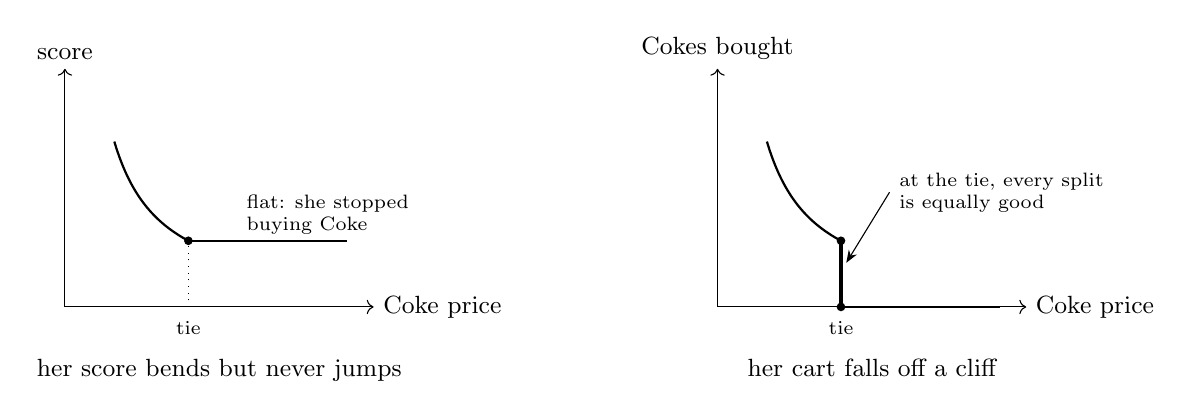
\begin{tikzpicture}[scale=1.12]
\begin{scope}
  \draw[->] (0,0) -- (3.5,0) node[right,font=\small] {Coke price};
  \draw[->] (0,0) -- (0,2.7) node[above,font=\small] {score};
  \draw[thick,domain=0.56:1.40,samples=70] plot (\x, {1.05/\x});
  \draw[thick] (1.40,0.75) -- (3.20,0.75);
  \draw[dotted] (1.40,0) -- (1.40,0.75);
  \fill (1.40,0.75) circle (1.4pt);
  \node[font=\scriptsize,anchor=north] at (1.40,-0.05) {tie};
  \node[font=\scriptsize,anchor=west,align=left] at (1.95,1.05) {flat: she stopped\\ buying Coke};
  \node[font=\small,anchor=north,align=center] at (1.75,-0.48)
    {her score bends but never jumps};
\end{scope}
\begin{scope}[xshift=7.4cm]
  \draw[->] (0,0) -- (3.5,0) node[right,font=\small] {Coke price};
  \draw[->] (0,0) -- (0,2.7) node[above,font=\small] {Cokes bought};
  \draw[thick,domain=0.56:1.40,samples=70] plot (\x, {1.05/\x});
  \draw[very thick] (1.40,0.75) -- (1.40,0);
  \draw[thick] (1.40,0) -- (3.20,0);
  \fill (1.40,0.75) circle (1.4pt);
  \fill (1.40,0) circle (1.4pt);
  \node[font=\scriptsize,anchor=north] at (1.40,-0.05) {tie};
  \node[font=\scriptsize,anchor=west,align=left] (seg) at (1.95,1.30)
    {at the tie, every split\\ is equally good};
  \draw[-{Stealth[length=1.6mm]}] (seg.west) -- (1.46,0.50);
  \node[font=\small,anchor=north,align=center] at (1.75,-0.48)
    {her cart falls off a cliff};
\end{scope}
\end{tikzpicture}
\end{center}

Every result so far can be tested on this one formula, and doing so is more useful than reading the
proofs again.

\begin{enumerate}[leftmargin=*,itemsep=2pt]
\item \emph{Redenomination.} Multiply prices and income by $t$: the $t$ cancels top and bottom and
her score is unchanged. Proposition \ref{prop:hd0} holds.
\item \emph{Prices, weakly.} Her score is flat in the Coke price once Coke is the dearer one, which
is the flat stretch in the left panel. This is exactly why Proposition \ref{prop:mono} states the
price claim weakly.
\item \emph{Income, strictly.} Her score is $I$ over a fixed number, so it rises strictly with
income, matching the strict half of Proposition \ref{prop:mono}.
\item \emph{Averaging countries.} Her score is at most $K$ exactly when
$I \le K p_1$ and $I \le K p_2$, two straight-line conditions, so the set of situations she likes no
better than $K$ is convex. Theorem \ref{thm:qcx} holds even though her tastes have no strict
curvature at all.
\item \emph{Smooth score.} A minimum of two continuous functions is continuous. Property 4 holds.
\item \emph{Jumpy behaviour.} And yet her cart flips at the tie. Proposition \ref{prop:xcont} does
not apply to her, because she has no unique best basket there.
\end{enumerate}

\begin{snugshade}
\noindent\textbf{Flag on the lecture's own display.} L3 p.5 writes the tie case coordinate by
coordinate, as $x_1^* \in [0, I/p_1]$ and $x_2^* \in [0, I/p_1]$. Read literally that allows buying
nothing at all, or buying $I/p$ of each, neither of which is optimal. The correct statement is that
she splits her budget somehow: $x_1 + x_2 = I/p$ with both parts non-negative. The second display
also carries $p_1$ where $p_2$ belongs, which is harmless only because the case is $p_1 = p_2$.
\end{snugshade}
\section{The suitcase that is already packed}
\label{sec:q5}

\subsection{The scene}

You have packed a 20 kg suitcase as well as it can be packed. The airline then raises your allowance
to 21 kg. What is that extra kilo worth to you?

The honest answer is: the value of the best thing you left behind. You do not unpack and start over.
You add one item.

Now ask how you would compute the answer the hard way. You would re-solve the whole packing problem
at 21 kg, compare the two packings, and take the difference. That involves working out how the entire
packing changes, which is a large calculation, and almost all of it cancels because you were already
packed well.

\subsection{The claim in plain words}

When you are already at the top, moving does not help you, so you may ignore the fact that you will
move.

Write the maximized value as $M(a) = f(x^*(a), a)$, where $a$ is the weight limit. The chain rule
gives two terms:
\[
M'(a) = \underbrace{f_x\big(x^*(a),a\big) \cdot x^{*\prime}(a)}_{\text{how the packing changes}}
\ + \ \underbrace{f_a\big(x^*(a),a\big)}_{\text{the limit itself changed}} .
\]
The first term is the one we cannot compute, because $x^{*\prime}(a)$ is the derivative of the
solution. The envelope theorem says it is zero.

\subsection{The envelope theorem}

\begin{thm}[Envelope] Let $M(a) = \max_{x \ge 0} f(x,a)$ with solution $x^*(a)$. Then
\[
M'(a) = \frac{\partial f(x,a)}{\partial a} \bigg|_{x = x^*(a)} .
\]
Differentiate with respect to the parameter first, holding the choice fixed, and substitute the
solution afterward. \src{L3 pp.5--6}, \src{J\&R Thm A2.22}
\end{thm}

\skipnote
\begin{leftbar}
\small
The first term above vanishes, and the reason is complementary slackness. At each $a$,
\[
f_x\big(x^*(a),a\big) \cdot x^*(a) = 0, \qquad f_x \le 0, \qquad x^* \ge 0 .
\]
If the solution is interior, $x^*(a) > 0$ forces $f_x = 0$, so the product is zero. If the solution
sits at a corner and stays there nearby, $x^*$ is locally constant, so $x^{*\prime}(a) = 0$ and the
product is zero again. Either way only the direct term survives.
\end{leftbar}

For the consumer's problem the same statement applies to the Lagrangian
$\mathcal{L} = u(x) + \lambda[I - p \cdot x]$, giving
\[
\frac{\partial v}{\partial \alpha} = \frac{\partial \mathcal{L}}{\partial \alpha}
\bigg|_{x^*, \lambda^*} \qquad \text{for any parameter } \alpha \text{ in } (p,I).
\qquad \src{L3 p.6}
\]

\subsection{Where the name comes from}

Fix the packing at some $\hat x$ and ask what its value does as the weight limit changes. That is one
curve. Do it for every packing and you get a family of curves. The value function is the highest one
at each $a$, so it sits on top of the family and touches whichever member happens to be best there.
At a touching point the two are tangent, so their slopes agree. The slope of the fixed-packing curve
is easy, because the packing is not moving.

\begin{center}
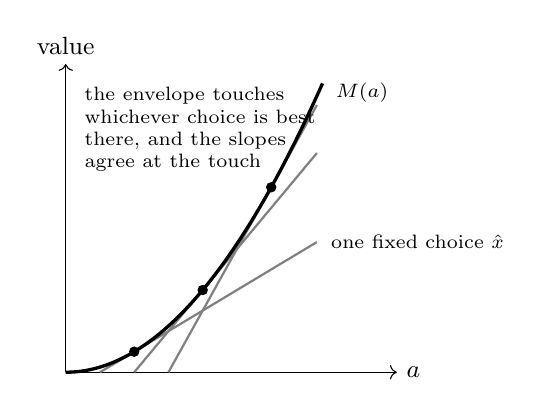
\begin{tikzpicture}[scale=1.45]
\draw[->] (0,0) -- (2.9,0) node[right,font=\small] {$a$};
\draw[->] (0,0) -- (0,2.7) node[above,font=\small] {value};
\draw[thick,gray,domain=0.30:2.2,samples=2] plot (\x, {0.6*\x-0.18});
\draw[thick,gray,domain=0.60:2.2,samples=2] plot (\x, {1.2*\x-0.72});
\draw[thick,gray,domain=0.90:2.2,samples=2] plot (\x, {1.8*\x-1.62});
\draw[very thick,domain=0:2.25,samples=80] plot (\x, {0.5*\x*\x});
\fill (0.6,0.18) circle (1.3pt);
\fill (1.2,0.72) circle (1.3pt);
\fill (1.8,1.62) circle (1.3pt);
\node[font=\scriptsize,anchor=west] at (2.28,2.45) {$M(a)$};
\node[font=\scriptsize,anchor=west] at (2.24,1.14) {one fixed choice $\hat{x}$};
\node[font=\scriptsize,anchor=north west,align=left] at (0.08,2.58)
  {the envelope touches\\ whichever choice is best\\ there, and the slopes\\ agree at the touch};
\end{tikzpicture}
\end{center}

\subsection{The lecture's exercise, with numbers}

The lecture sets $M(a) = \max x_1 x_2$ subject to $a - 2x_1 - 4x_2 \ge 0$ and asks for $M'(a)$ by
both methods \src{L3 p.7}.

\emph{Solve it.} With $\mathcal{L} = x_1 x_2 + \lambda[a - 2x_1 - 4x_2]$, the first-order conditions
are $x_2 = 2\lambda$ and $x_1 = 4\lambda$, and the constraint binds, so $16\lambda = a$ and
\[
\lambda^* = \frac{a}{16}, \qquad x_1^* = \frac{a}{4}, \qquad x_2^* = \frac{a}{8},
\qquad M(a) = \frac{a^2}{32}.
\]

\emph{The hard way.} $M'(a) = a/16$, obtained by substituting the solution and differentiating.

\emph{The envelope way.} $\partial \mathcal{L} / \partial a = \lambda$, so $M'(a) = \lambda^* = a/16$.
The solution never had to be differentiated.

\emph{Check it against actual numbers.} At $a = 16$ the value is 8. The envelope theorem says the
next unit of the resource is worth $\lambda^* = 1.00$.

\begin{center}
\begin{tabular}{@{}llll@{}}
\toprule
\textbf{Step in $a$} & \textbf{Actual change in value} & \textbf{Envelope prediction} & \textbf{Error} \\
\midrule
$16 \to 17$ & $9.031 - 8 = 1.031$ & $1.000$ & 3\% \\
$16 \to 16.1$ & $8.1003 - 8 = 0.1003$ & $0.1000$ & 0.3\% \\
\bottomrule
\end{tabular}
\end{center}

The prediction is not exactly right for a finite step and gets better as the step shrinks, which is
what ``to first order'' means. It is a derivative, not a forecast.

\fwd{L4} The same theorem applied to the mirror problem gives Shephard's lemma,
$x_i^h = \partial e / \partial p_i$, which the lecture proves in one line as immediate by the envelope
theorem \src{L4 p.4}.

\fwd{L5} The Slutsky equation is built by differentiating a duality identity and then substituting
Shephard's lemma \src{L5 p.2}. Every step in it is an envelope result. Lecture 3 does not so much
introduce a tool as point an existing tool in a new direction.

\section{Reading the shopping list off the pain}
\label{sec:q6}

\subsection{The scene: thirty cents}

Coffee goes up by one cent, from \$2.00 to \$2.01. Our consumer's score falls from 24.4949 to
24.4338, a drop of 0.0611.

Separately, hand her one extra dollar. Her score rises by 0.204.

Now divide. The penny on coffee hurt her by $0.0611 / 0.204 = 0.30$ dollars' worth of score. So the
price rise cost her thirty cents.

And she buys thirty coffees. A penny on each of thirty coffees is thirty cents.

\subsection{The claim in plain words}

A small price rise hurts you by exactly what you were spending on that good. So if you can measure
how much people are hurt by price changes, and how much they value money, you can read off what they
buy without ever asking them.

That is Roy's identity, and it is the reason the whole sequence was built. Preferences are invisible.
This formula goes from something you can estimate to something you want to know.

\begin{lem}[Roy's identity, the lecture's Lemma 3.1] \label{lem:roy}
If $u$ is differentiable, strictly increasing and strictly quasi-concave, then
\[
x_i^*(p,I) = - \frac{\partial v / \partial p_i}{\partial v / \partial I} .
\qquad \src{L3 p.6}, \src{J\&R Thm 1.6.6}
\]
\end{lem}

\skipnote
\begin{leftbar}
\small
Apply the envelope theorem to the Lagrangian
$\mathcal{L} = u(x) + \lambda(I - p \cdot x)$ in each parameter, holding $x$ and $\lambda$ fixed and
evaluating at the solution. For income the bracket contributes $\lambda$, so
\[
\frac{\partial v}{\partial I} = \lambda^* > 0,
\]
the sign being Lecture 2's conclusion that if more is always better then an extra dollar is worth
something \src{L2 p.7}. For a price the bracket contributes $-x_i$, so
\[
\frac{\partial v}{\partial p_i} = - \lambda^* x_i^* .
\]
Dividing the second by the first and changing sign, the $\lambda^*$ cancels and leaves $x_i^*$.
\end{leftbar}

Going the direct route instead would mean differentiating $v = u(x^*(p,I))$ through the chain rule,
producing one unknown term per good. The lecture describes that as long and complicated and stops
\src{L3 p.7}.

\subsection{Why a ratio, and why a minus sign}

Both of these follow from things already established, so neither needs memorizing.

\textbf{The minus sign} is because a price rise lowers her score, so $\partial v / \partial p_i$ is
negative, while a quantity of coffee is positive. The sign flip converts one to the other.

\textbf{The ratio} is a unit conversion. The 0.0611 and the 0.204 are both measured in her utility
scale, which \S\ref{sec:q1}.5 established is arbitrary. Relabel her utility as $1000u$ and both
numbers multiply by a thousand. Dividing one by the other cancels the arbitrary factor and leaves a
quantity of coffee, which is real.

Here is that claim run on her actual numbers. Use $\ln u$ instead of $u$ as her utility function,
which Lecture 1 says represents the same preferences \src{L1 p.5}.

\begin{center}
\begin{tabular}{@{}lccc@{}}
\toprule
 & \textbf{Her score} & $\partial / \partial p_1$ & $\partial / \partial I$ \\
\midrule
Using $u = \sqrt{x_1 x_2}$ & 24.4949 & $-6.1237$ & $0.20412$ \\
Using $\ln u$ & 3.1985 & $-0.25$ & $0.008333$ \\
\midrule
Roy's ratio & & \multicolumn{2}{c}{\textbf{30 coffees, both times}} \\
\bottomrule
\end{tabular}
\end{center}

Every input changed. The answer did not. The non-invariant object and the invariant one live in the
same formula, and that is the whole point of this question. J\&R Exercise 1.33 states the general
version: any strictly increasing transform of an indirect utility function is itself a perfectly good
indirect utility function.

\bwd{L1} You have met this exact cancellation before. Lecture 1 argued that marginal utility means
nothing on its own, because relabeling $u$ scales it, while the marginal rate of substitution means
something, because it is a ratio in which the scaling cancels \src{L1 pp.15--18}. Roy's identity is
that same argument one level up. If you can say why the MRS is invariant, you can say why Roy's
identity is.

\subsection{Why Shephard's lemma has no ratio and no minus sign}

Lecture 4 produces $x_i^h = \partial e / \partial p_i$, which looks like a simpler cousin of Roy
\src{L4 p.4}. It is simpler for two reasons, both already on the table.

\begin{center}
\begin{tabular}{@{}p{0.24\textwidth} p{0.34\textwidth} p{0.34\textwidth}@{}}
\toprule
 & \textbf{Roy, from Lecture 3} & \textbf{Shephard, from Lecture 4} \\
\midrule
The value is measured in & her arbitrary utility scale & dollars \\
So it needs converting? & yes, divide by $\partial v / \partial I$ & no, already in dollars \\
A price rise makes the value & fall & rise \\
So it needs a sign flip? & yes & no \\
\bottomrule
\end{tabular}
\end{center}

\subsection{A check that hands back the budget constraint}

\begin{prop} If $v$ is differentiable and HD0, if $\partial v / \partial I > 0$, and if Roy's identity
holds, then $p \cdot x^*(p,I) = I$.
\end{prop}

\skipnote
\begin{leftbar}
\small
Euler's equation \eqref{eq:eulerv} for the HD0 function $v$ says
$\sum_i v_{p_i} p_i + v_I \, I = 0$. Roy's identity rearranged says
$v_{p_i} = - x_i^* \, v_I$. Substituting,
\[
- v_I \sum_i p_i x_i^* + v_I \, I = 0
\quad \Longrightarrow \quad
v_I \big( I - p \cdot x^* \big) = 0,
\]
and since $v_I > 0$ the bracket vanishes.
\end{leftbar}

\textbf{Why this is worth running.} Lecture 2 proved that she spends everything, by a direct argument
from the fact that more is better \src{L2 p.5}. Here the same conclusion drops out of two properties
of the welfare function. Two independent routes to one answer is the best evidence available that
nothing has gone wrong, and on our consumer it is the statement that $2 \times 30 + 3 \times 20 = 120$.

Use it as a habit. Whenever you compute a $v$ from scratch, check that it is unchanged by a
redenomination and that Roy plus Euler returns the budget constraint. Both checks take seconds and
catch algebra errors that reading the work again will not.

\subsection{What breaks}

Each of the three hypotheses in Lemma \ref{lem:roy} is load-bearing, and each failure has a face you
have already met.

\textbf{Drop ``more is always better''.} The consumer from \S\ref{sec:q2}.4 whose ideal basket costs
\$17 out of her \$120 has $\partial v / \partial I = 0$ \src{RS2 Q2.3}. Roy's identity asks you to
divide by zero. J\&R states the identity with the explicit proviso that this derivative is nonzero
\src{J\&R p.29}.

\textbf{Drop unique best basket, and differentiability goes with it.} The soda drinker at the tie has
a whole line of best baskets, and her score has a kink at exactly that price, so there is no
derivative to take \src{L3 p.5}. These two failures happen at the same point, and that is not a
coincidence: Roy's identity is supposed to return one number, and where there is no single best
basket there is no single number for it to return.

Away from the tie it works. With Coke cheaper, $v = I/p_1$, and
\[
- \frac{\partial v / \partial p_1}{\partial v / \partial I} = \frac{I/p_1^2}{1/p_1} = \frac{I}{p_1},
\qquad
- \frac{\partial v / \partial p_2}{\partial v / \partial I} = 0,
\]
which says she spends everything on Coke and buys no Pepsi. Correct.

\begin{snugshade}
\noindent\textbf{Flag on a strict inequality.} L3 p.8 writes
$\partial v / \partial p_i = -\lambda^* x_i^* < 0$. That is strict only where she actually buys good
$i$. The soda drinker facing dear Coke has $x_1^* = 0$, and her $\partial v / \partial p_1$ is zero,
not negative. J\&R states the corresponding property weakly for this reason \src{J\&R p.29}.
\end{snugshade}
\section{Where this goes}

\subsection{Lecture 4 asks the question backwards}

Lecture 3 fixed her budget and asked how well off she ends up. Lecture 4 fixes how well off she is
and asks what it costs \src{L4 p.1}:
\[
e(p, u^0) = \min_x \ p \cdot x \quad \text{subject to} \quad u(x) \ge u^0, \ x \ge 0 .
\]

On our consumer: she currently scores 24.49 at prices \$2 and \$3, and it costs her \$120. If coffee
rose to \$2.50, what would she need to be handed to stay at 24.49? That question is the expenditure
function, and it is the right way to measure the damage from a price rise, because the answer comes
out in dollars.

\textbf{What carries over unchanged.} The two lemmas of \S\ref{sec:q2}. Demanding a higher standard
of living shrinks the set of acceptable baskets and so can only raise the bill; a higher price raises
the bill for every basket. Those are Lemmas \ref{lem:mv} and \ref{lem:bmove} again, pointed at a
different constraint set, and they give properties 3 and 4 of the expenditure function \src{L4 p.2}.
Berge reappears verbatim as property 2, with the same upgrade from strict curvature that Proposition
\ref{prop:xcont} gave here. The envelope theorem reappears as Shephard's lemma.

\textbf{What is new.} The set of baskets that are good enough is closed but not bounded, so existence
cannot come from Weierstrass and the argument runs on the objective instead \src{L4 p.2}. The bill is
\emph{concave} in prices, and with that comes the machinery of negative semi-definite Hessians,
Young's theorem, and the substitution matrix \src{L4 pp.3--6}.

\textbf{Three things that look the same and are not.}

\begin{itemize}
\item Quasi-convex $v$ and concave $e$ are not a matched pair. Concavity signs second derivatives and
quasi-convexity signs nothing, which is why the substitution-matrix theory has no counterpart in
Lecture 3.
\item Roy and Shephard differ for the two reasons in the table in \S\ref{sec:q6}.4, both of which come
down to $e$ being measured in dollars.
\item The homogeneity degrees differ: $v$ and $x^*$ are degree zero in prices and income together,
$e$ is degree one in prices, and $x^h$ is degree zero in prices with no income argument at all,
because the compensation is carried by $u^0$ \src{L2 p.4}, \src{L4 p.2}.
\end{itemize}

\subsection{Lecture 5 joins the two}

Lecture 5 shows that $v$ and $e$ undo each other: the cost of reaching the standard she actually
reaches is her income, and the standard reachable on that budget is the standard she actually
reaches \src{L5 p.1}. The proof uses continuity and ``more is better'' and nothing else, which are
the same two hypotheses that have been doing this work since \S\ref{sec:q2}.

The payoff is the Slutsky equation \src{L5 p.2}, which splits the effect of a price rise into two
parts: the part where she substitutes toward whatever got relatively cheaper, and the part where she
is simply poorer. On our consumer, a coffee price rise reduces coffee for both reasons, and Lecture 5
shows the two halves are exactly equal for Cobb-Douglas \src{L5 p.4}. The classification into normal
and inferior goods, and the possibility of a good whose demand rises with its price, all come out of
which way the second part points.

\textbf{One thing that looks the same and is not.} The substitution part is always negative. The
total effect is not, and confusing the two is the error behind most wrong answers about Giffen goods
\src{L5 p.3}.

\subsection{Reading list}

\begin{itemize}
\item The expenditure function and its properties, J\&R \S1.4.2, Theorem 1.7.
\item How $v$ and $e$ relate, J\&R \S1.4.3, Theorems 1.8 and 1.9.
\item Homogeneity and budget balancedness as testable restrictions, J\&R \S1.5.1, Theorem 1.10.
\item Income and substitution effects, J\&R \S1.5.2, Theorems 1.11 to 1.16.
\item Elasticities and aggregation, J\&R \S1.5.3, Definition 1.6 and Theorem 1.17.
\end{itemize}

\section{Items to confirm with the TA}

None of these is in the notes as written, and each could cost marks if you reproduce the lecture
version on an exam.

\begin{enumerate}[leftmargin=*,itemsep=3pt]
\item \textbf{Property 1 has no proof.} L3 p.1 asserts that $v$ is homogeneous of degree zero and
gives no argument at all. The two-line version is in \S\ref{sec:q2}.2.

\item \textbf{The quasi-convexity proof stops halfway.} L3 p.4 proves that the averaged budget set
sits inside the union of the two extremes, then says it suffices. The step from that containment to
the inequality on scores is not given. It is Step 2 in \S\ref{sec:q3}.3.

\item \textbf{Proposition 3.1 is unproved.} L3 p.4 marks the continuity of demand ``Proof. Omitted.''
The argument in \S\ref{sec:q4}.4 needs Property 4 as an input, which is worth knowing because it
means the two results cannot be quoted independently.

\item \textbf{The tie case is written wrongly.} L3 p.5 gives the solution for linear utility
coordinate by coordinate, which read literally permits buying nothing. It also carries $p_1$ where
$p_2$ belongs in the second display.

\item \textbf{A strict inequality that should be weak.} L3 p.8 writes
$\partial v / \partial p_i = -\lambda^* x_i^* < 0$, which fails wherever the consumer buys none of
good $i$.

\item \textbf{Weak against strict monotonicity.} L3 p.1 states all the monotonicity claims weakly.
J\&R Theorem 1.6 makes the income claim strict and leaves the price claim weak. The lecture also
assumes only that $u$ is continuous, where J\&R assumes continuous and strictly increasing. Since
Roy's identity needs the income derivative to be nonzero, the strict version is the one that matters
downstream.

\item \textbf{A notation collision.} The letter $B$ is the better-than set in Lecture 1 and the
budget set from Lecture 2 onward, and both appear in discussions of convexity.
\end{enumerate}

\end{document}
